\documentclass[12pt]{article}

\input{../../Latex_Common/skinnerr_latex_preamble_asen5417.tex}

%%
%% DOCUMENT START
%%

\begin{document}

\pagestyle{fancyplain}
\lhead{}
\chead{}
\rhead{}
\lfoot{ASEN 5417: Homework 2}
\cfoot{\thepage}
\rfoot{Ryan Skinner}

\noindent
{\Large Homework 2}
\hfill
{\large Ryan Skinner}
\\[0.5ex]
{\large ASEN 5417: Numerical Methods}
\hfill
{\large Due 2015/09/17}\\
\hrule
\vspace{6pt}

%%%%%%%%%%%%%%%%%%%%%%%%%%%%%%%%%%%%%%%%%%%%%%%%%
%%%%%%%%%%%%%%%%%%%%%%%%%%%%%%%%%%%%%%%%%%%%%%%%%
\section{Introduction} %%%%%%%%%%%%%%%%%%%%%%%%%%
%%%%%%%%%%%%%%%%%%%%%%%%%%%%%%%%%%%%%%%%%%%%%%%%%
%%%%%%%%%%%%%%%%%%%%%%%%%%%%%%%%%%%%%%%%%%%%%%%%%

We solve the following problems to better understand numerical techniques for solving initial value problems governed by ordinary differential equations. As will be described in the methods section, our tools primarily consist of second- (RK2) and fourth-order (RK4) Runge-Kutta methods, as well as Euler stability analysis.

\subsection{Problem 1}

Equations of motion for a rocket's vertical speed $v$ can be written as
\begin{equation}
(m_c + m_p) \frac{dv}{dt} = -(m_c + m_p) g + \dot{m}_p v_e - \tfrac{1}{2} \rho v \norm{v} A C_D
,
\label{eq:rocket}
\end{equation}
where $z$ is the vertical coordinate, $v = dz/dt$ is the vertical speed, and
\begin{equation*}
\begin{aligned}
m_c &= 51.02 \text{ kg} &&\text{(rocket casing mass)} \\
g &= 9.8 \text{ m/s}^2 &&\text{(gravitational acceleration)} \\
\rho &= 1.23 \text{ kg/m}^3 &&\text{(air density)} \\
A &= 0.1 \text{ m}^2 &&\text{(maximum cross-sectional area)} \\
v_e &= 360 \text{ m/s} &&\text{(exhaust speed)} \\
C_D &= 0.15 &&\text{(drag coefficient)} \\
m_{p0} &= 102.04 \text{ kg} &&\text{(initial propellant mass)}
.
\end{aligned}
\end{equation*}
Furthermore, the instantaneous propellant mass at time $t$ is given by
\begin{equation}
m_p(t) = m_{p0} - \int_0^t \dot{m}_p dt
,
\end{equation}
and the time-varying burn rate is
\begin{equation}
\dot{m}_p =
\frac{m_{p0}}{4}
\cdot
\begin{cases}
t     & 0 \le t \le 1 \\
1     & 1 \le t \le 4 \\
5 - t & 4 \le t \le 5 \\
0     & 5 \le t
.
\end{cases}
\end{equation}

Use a second-order Runge-Kutta (RK2) integrator with $\Delta t = 0.1 \text{ s}$ to plot $z(t)$ and $v(t)$. Use these plots to find the maximum speed, and the height and time at which it is reached; the maximum height, and the time at which it is reached; and the time and velocity when the rocket hits the ground. Check these results with those obtained from \textsc{Matlab}'s \lstinline|ode45| solver.

This problem is fairly straight-forward. An RK2 scheme is relatively easy to implement, but we will need to be careful when accounting for the time-dependence of $m_p$. Furthermore, though it is not stated in the problem, when $m_p$ reaches zero, the thrust term involving the exhaust speed $v_e$ in \eqref{eq:rocket} needs to ``turn off.'' Lastly, it would be un-physical for the rocket to initially fall through the launch pad before thrust overcomes gravity, and we must account for this when coding the solution.

\subsection{Problem 2}

Consider the stream function for a two-dimensional jet in self-similar form, which can be written as
\begin{equation}
f''(\eta) + f(\eta) f'(\eta) = 0 ,\qquad
f(0) = 0 ,\qquad
f'(0) = 1 ,\qquad
\Rightarrow \;
f''(0) = 0
.
\label{eq:prob2}
\end{equation}
The velocities in the jet can be obtained via
\begin{equation}
\frac{U}{U_0} = f'(\eta) ,\qquad
\frac{V}{U_0} = \eta f'(\eta) - \tfrac{1}{2} f(\eta)
.
\label{eq:prob2_velocities}
\end{equation}
Using numerical integration for $0 \le \eta \le 4$, with a step size of $\Delta \eta = 0.05$, plot the quantities $U/U_0$, $V/V_0$, and $f$ as functions of $\eta$. Perform this analysis with both the second- (custom) and fourth-order (\lstinline|ode45|) Runge-Kutta methods, and compare their performance. Both solutions may be compared to those obtained from the best-fit expression
\begin{equation}
f'(\eta) = \exp(\gamma \eta^2)
,
\label{eq:prob2_bestfit}
\end{equation}
where $\gamma = -0.0692$.

\subsection{Problem 3}

Show that the equation
\begin{equation}
y'' = -\frac{19}{4} y - 10 y' ,\qquad
y(0) = -9 ,\qquad
y'(0) = 0 ,\qquad
\Rightarrow \;
y''(0) = \frac{171}{4}
\label{eq:prob3}
\end{equation}
is moderately stiff. Use Euler stability analysis to estimate the largest step size $h_\tmax$ for which the Runge-Kutta method will be stable. Then confirm this estimate by computing $y(10)$ using the fourth-order Runge-Kutta method with $h = \{ \tfrac{1}{2} h_\tmax, 2 h_\tmax\}$. Compare these solutions with the analytical solution.

%%%%%%%%%%%%%%%%%%%%%%%%%%%%%%%%%%%%%%%%%%%%%%%%%
%%%%%%%%%%%%%%%%%%%%%%%%%%%%%%%%%%%%%%%%%%%%%%%%%
\section{Methodology} %%%%%%%%%%%%%%%%%%%%%%%%%%%
%%%%%%%%%%%%%%%%%%%%%%%%%%%%%%%%%%%%%%%%%%%%%%%%%
%%%%%%%%%%%%%%%%%%%%%%%%%%%%%%%%%%%%%%%%%%%%%%%%%

\subsection{Problem 1}

We first re-write the system of equations governing rocket altitude as
\begin{equation}
\begin{aligned}
\frac{dz}{dt} &= f(t,z,v) &&= v
\\
\frac{dv}{dt} &= g(t,z,v) &&= \underbrace{-g + T \frac{\dot{m}_p v_e}{(m_c + m_p)}}_{\alpha(t)} + \underbrace{\frac{- \rho A C_D}{2 (m_c + m_p)}}_{\beta(t)} v \norm{v}
,
\end{aligned}
\label{eq:rocket_rewritten}
\end{equation}
where $\alpha$ and $\beta$ are constants that directly depend only on time, and
\begin{equation}
T =
\begin{cases}
1 & 0 \le t < 5 \\
0 & \text{all other $t$}
\end{cases}
\end{equation}
toggles the thrust term on and off based on whether the rocket engines are on. In the \textsc{Matlab} code, the functions that calculate $\alpha(t)$ and $\beta(t)$ call subsequent functions to calculate $m_p(t)$ and $\dot{m}_p(t)$.

Given the initial values of our variables at $t=0$, the 2\nd-order Runge-Kutta method allows us to integrate the system of equations \eqref{eq:rocket_rewritten} with respect to time using a time step $h$. At a given time $t_n$, the velocity and position at the next time step, $v_{n+1}$ and $z_{n+1}$, can be approximated by, at each successive time step, calculating
\begin{equation}
\begin{aligned}
k_1 &= h f(t_n, z_n, v_n)
\\
l_1 &= h g(t_n, z_n, v_n)
\\
k_2 &= h f(t_n + \tfrac{1}{2} h, z_n + \tfrac{1}{2} k_1, v_n + \tfrac{1}{2} l_1)
\\
l_2 &= h g(t_n + \tfrac{1}{2} h, z_n + \tfrac{1}{2} k_1, v_n + \tfrac{1}{2} l_1)
\end{aligned}
\end{equation}
and then updating the next step's values of $z$ and $v$ as
\begin{equation}
\begin{aligned}
z_{n+1} &= z_n + k_2
\\
v_{n+1} &= v_n + l_2
.
\end{aligned}
\end{equation}

For early time steps, say $t < 3$, we ensure that the rocket does not fall through the launch pad by setting $v_{n+1}$ and $z_{n+1}$ to zero if they are negative after the RK2 iteration.

\subsection{Problem 2}

We are able to use an analogous method to Problem 1 for the RK2 integrator, and we choose \textsc{Matlab}'s \lstinline|ode45| function as our higher-order integrator. Normalized velocities are calculated at each value of $\eta$ using the results of integration according to \eqref{eq:prob2_velocities}. The best-fit expression \eqref{eq:prob2_bestfit} has an analytical solution for $f$ given by
\begin{equation}
f(\eta) = \sqrt{\pi / 4 \gamma} \erf(\sqrt{\gamma} \eta)
\end{equation}
where constant of integration for $f(\eta)$ must be zero to match the initial condition. We integrate the variables $f(\eta)$ and $f'(\eta)$, and at each time step use the definition from \eqref{eq:prob2} to calculate $f''(\eta)$.

\subsection{Problem 3}

An analytical solution for \eqref{eq:prob3} exists, and we find it by assuming that $y(t)$ has the form $\exp(\lambda t)$. The values of $\lambda$ allow us to determine how stiff the ODE is.

Euler stability analysis can be performed on the system of equations
\begin{equation}
\frac{d}{dt}
\begin{bmatrix}
y \\
y'
\end{bmatrix}
=
\mathbf{A}
\begin{bmatrix}
y \\
y'
\end{bmatrix}
, \qquad
\mathbf{A}
=
\begin{bmatrix}
0 & 1 \\
-\frac{19}{4} & -10
\end{bmatrix}
,
\end{equation}
by finding the eigenvalues $\lambda_i$ of $\mathbf{A}$. For a forward Euler method at least, the maximum step size for which a numerical solution is stable is given by
\begin{equation}
h_\tmax < \frac{2}{\max_i\norm{\lambda_i}}
.
\end{equation}

For the 4\th-order Runge-Kutta method, at each successive time step $t_n$ we calculate
\begin{equation}
\begin{aligned}
\mathbf{k}_1 &= h f(t_n, \mathbf{y}_n)
\\
\mathbf{k}_2 &= h f(t_n + \tfrac{1}{2} h, \mathbf{y}_n + \tfrac{1}{2} \mathbf{k}_1)
\\
\mathbf{k}_3 &= h f(t_n + \tfrac{1}{2} h, \mathbf{y}_n + \tfrac{1}{2} \mathbf{k}_2)
\\
\mathbf{k}_4 &= h f(t_n + \tfrac{1}{2} h, \mathbf{y}_n + \mathbf{k}_3)
\end{aligned}
\end{equation}
where $\mathbf{y}_n$ is a vector of solution variables evaluated at time $t_n$, and $\mathbf{k}_i$ is a vector of intermediate values for each variable represented by $\mathbf{y}_n$. Finally, we update the next step's values of $z$ and $v$ as
\begin{equation}
\begin{aligned}
\mathbf{y}_{n+1} &= \mathbf{y}_n + \tfrac{1}{6} \left( \mathbf{k}_1 + 2 \mathbf{k}_2 + 2 \mathbf{k}_3 + \mathbf{k}_4 \right)
.
\end{aligned}
\end{equation}

%%%%%%%%%%%%%%%%%%%%%%%%%%%%%%%%%%%%%%%%%%%%%%%%%
%%%%%%%%%%%%%%%%%%%%%%%%%%%%%%%%%%%%%%%%%%%%%%%%%
\section{Results} %%%%%%%%%%%%%%%%%%%%%%%%%%%%%%%
%%%%%%%%%%%%%%%%%%%%%%%%%%%%%%%%%%%%%%%%%%%%%%%%%
%%%%%%%%%%%%%%%%%%%%%%%%%%%%%%%%%%%%%%%%%%%%%%%%%

\subsection{Problem 1}

Plots of the velocity and altitude time histories are presented in \figref{fig:rocket_plots}. Statistics on notable flight events are shown in Table~\ref{tbl:rocket}.

\begin{figure}[h!]
\begin{center}
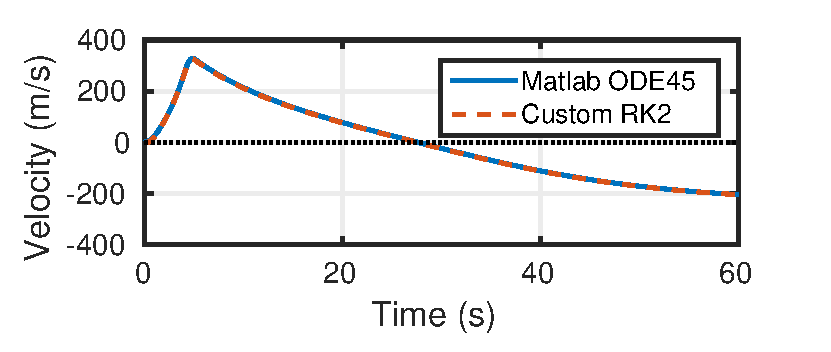
\includegraphics[width=0.49\textwidth]{rocket_velocity.eps}
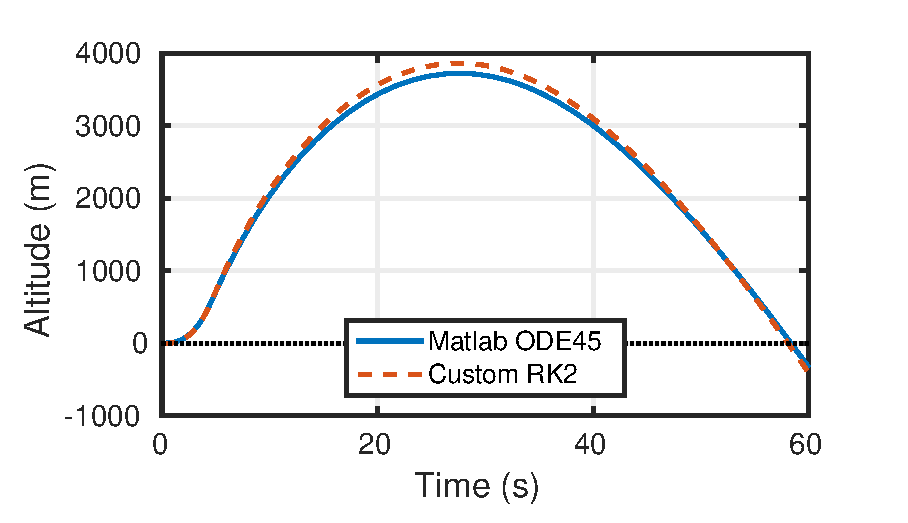
\includegraphics[width=0.49\textwidth]{rocket_altitude.eps}
\\[6pt]
\caption{Comparison of our own 2\nd-order Runge-Kutta scheme to \textsc{Matlab}'s \lstinline|ode45| solver, for the rocket velocity and altitude.}
\label{fig:rocket_plots}
\end{center}
\end{figure}

\begin{table}[h!]
\centering
\begin{tabular}{llllllll}
\toprule
Integrator   & \multicolumn{3}{c}{Max Velocity} & \multicolumn{2}{c}{Max Altitude} & \multicolumn{2}{c}{Crash} \\
\midrule
~            & Time & Velocity & Altitude       & Time         & Altitude & Time  & Velocity \\
Custom RK2                        & 4.80 & 325.74   & 653.47  & 27.50  & 3861.61  & 58.06 & -199.79  \\
\textsc{Matlab} \lstinline|ode45| & 4.80 & 328.71   & 648.04  & 27.74  & 3723.21  & 58.34 & -200.19 \\
\bottomrule
\end{tabular}
\\[6pt]
\caption{Comparison of notable flight events between integration methods.}
\label{tbl:rocket}
\end{table}

\subsection{Problem 2}

\begin{figure}[t]
\begin{center}
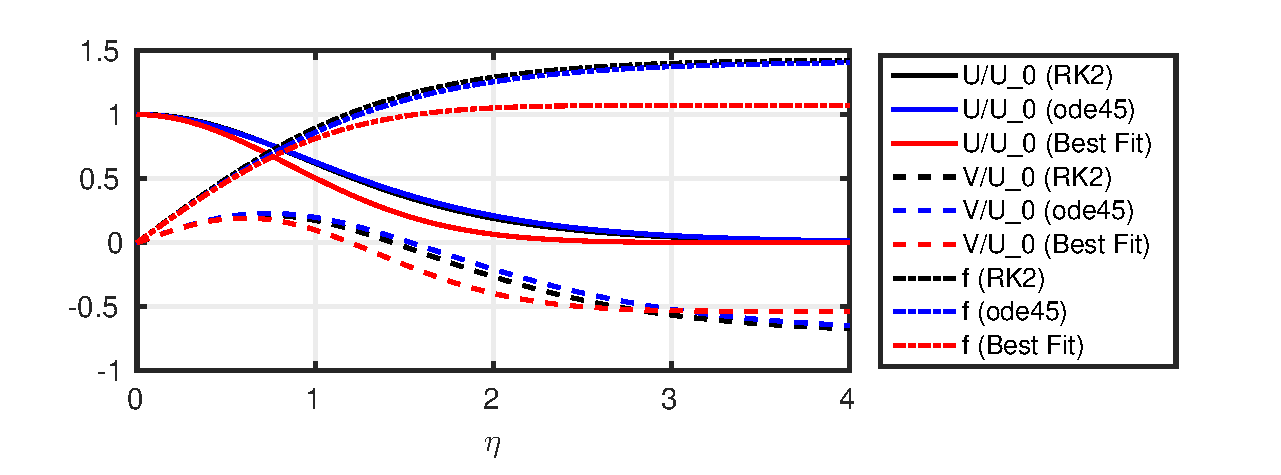
\includegraphics[width=\textwidth]{prob2.eps}
\\
\caption{Plots of the stream function $f$ and the normalized velocities $U/U_0$ and $V/V_0$ as a function of the similarity variable $\eta$, using two different integration methods and the experimentally-determined best fit for $f'(\eta)$.}
\label{fig:prob2}
\end{center}
\end{figure}

Results of for the stream function and normalized velocities as a function of the similarity variable $\eta$ are presented in \figref{fig:prob2}.

\subsection{Problem 3}

The analytical solution to \eqref{eq:prob3} is
\begin{equation}
y = -\frac{19}{2} \exp \left( \frac{-x}{2} \right) + \frac{1}{2} \exp \left( \frac{-19x}{2} \right)
.
\label{eq:prob3_analytic}
\end{equation}
Since the first exponent has a characteristic time scale of 2, and the second has a characteristic time scale of 2/19, we conclude that the ODE is moderately stiff. Put simply, the second exponential term decays approximately $20\times$ more rapidly than the first, and it will be somewhat difficult to capture both time scales accurately with a fixed step size.

Euler stability analysis yields eigenvalues of $\lambda = \{ \tfrac{-1}{2}, \tfrac{-19}{2} \}$, and thus our estimate of the largest value of $h$ for which we expect the solution to be stable is
\begin{equation}
h_\tmax = \frac{4}{19}
.
\end{equation}

Values of $y(10)$ are shown in Table~\ref{tbl:prob3}.

\begin{figure}[h!]
\floatbox[{\capbeside\thisfloatsetup{capbesideposition={right,center},capbesidewidth=8cm}}]{table}[\FBwidth]
{\caption{Comparison of $y(10)$ between the analytical solution and the 4\th-order Runge-Kutta method with different step sizes.}\label{tbl:prob3}}
{
	\begin{tabular}{ll}
	\toprule
	Method & $y(10)$ \\
	\midrule
	Analytical                  & -0.0640 \\
	RK4 ($\tfrac{1}{2}h_\tmax$) & -0.0419 \\
	RK4 ($2h_\tmax$)            & 8.2059$\times10^{13}$ \\
	\bottomrule
	\end{tabular}
}
\end{figure}

%%%%%%%%%%%%%%%%%%%%%%%%%%%%%%%%%%%%%%%%%%%%%%%%%
%%%%%%%%%%%%%%%%%%%%%%%%%%%%%%%%%%%%%%%%%%%%%%%%%
\section{Discussion} %%%%%%%%%%%%%%%%%%%%%%%%%%%%
%%%%%%%%%%%%%%%%%%%%%%%%%%%%%%%%%%%%%%%%%%%%%%%%%
%%%%%%%%%%%%%%%%%%%%%%%%%%%%%%%%%%%%%%%%%%%%%%%%%

\subsection*{Problem 1}

Using both integration strategies, we physically see the rocket accelerate at an increasing rate as propellant is burned, and then decelerate as the rocket engine shuts down and the forces of gravity and air drag dominate its dynamics. 

Agreement of time-histories of rocket velocity and altitude is strong between the 2\nd-order Runge-Kutta method we implemented and \textsc{Matlab}'s own \lstinline|ode45| solver. This holds true both visually and quantitatively, based on \figref{fig:rocket_plots} and Table~\ref{tbl:rocket} respectively. Errors between methods are within 3\% for time, within 1\% for velocity, and within 9\% for altitude.

Any disagreement can be attributed to two phenomena. First, \textsc{Matlab}'s integrator uses an adaptive time-step coupled with a higher-order integration scheme. It is thus able to capture the rocket's take-off behavior more accurately. Since the propellant-burning phase heavily influences the maximum altitude achieved, any small inaccuracies from the RK2 method during that phase will throw off the altitude profile compared to the more-accurate \lstinline|ode45| solution. Second, position errors are more pronounced than velocity errors, because errors from the velocity calculations are compounded when estimating the altitude at each time step.

\subsection{Problem 2}

Differences between the Runge-Kutta methods used are qualitatively small. This is likely due to the stream function $f(\eta)$ having relatively small curvature over the domain of interest. If curvatures were more pronounced, the higher-order method would approximate the solution much more accurately.

The experimental best-fit expression for $f'(\eta)$ matches the velocities $U/U_0$ and $V/V_0$ fairly well, but since it is only an exponential function fit to experimental data, it struggles to capture the true behavior of the governing ODE (which is not \emph{exactly} exponential). All things considered, it does a decent job of matching the normalized velocities, though agreement is not perfect.

\subsection{Problem 3}

Since we are using an RK4 method instead of an Euler method, Euler stability analysis is only a guide. If we violate the $h_\tmax$ criterion, numerical instabilities will persist. If not, however, there is still no guarantee the solution will be stable. This is borne out in our results (Table~\ref{tbl:prob3}), as the solution with $h=2h_\tmax$ diverges rapidly. Fortunately, using a step size of $h=\tfrac{1}{2}h_\tmax$ does not diverge, and produces a value of $y(10)$ within 35\% of the analytical value. We would likely need to reduce the step size considerably to get below 1\% error, since the governing equation is moderately stiff. This is a situation in which an adaptive step size may be appropriate.

%%%%%%%%%%%%%%%%%%%%%%%%%%%%%%%%%%%%%%%%%%%%%%%%%
%%%%%%%%%%%%%%%%%%%%%%%%%%%%%%%%%%%%%%%%%%%%%%%%%
\section{References} %%%%%%%%%%%%%%%%%%%%%%%%%%%%
%%%%%%%%%%%%%%%%%%%%%%%%%%%%%%%%%%%%%%%%%%%%%%%%%
%%%%%%%%%%%%%%%%%%%%%%%%%%%%%%%%%%%%%%%%%%%%%%%%%

No external references were used other than the course notes for this assignment.

%%%%%%%%%%%%%%%%%%%%%%%%%%%%%%%%%%%%%%%%%%%%%%%%%
%%%%%%%%%%%%%%%%%%%%%%%%%%%%%%%%%%%%%%%%%%%%%%%%%
\section*{Appendix: MATLAB Code} %%%%%%%%%%%%%%%%
%%%%%%%%%%%%%%%%%%%%%%%%%%%%%%%%%%%%%%%%%%%%%%%%%
%%%%%%%%%%%%%%%%%%%%%%%%%%%%%%%%%%%%%%%%%%%%%%%%%

The following code listings generate all figures presented in this homework assignment.

\includecode{Problem_1.m}
\includecode{Problem_2.m}
\includecode{Problem_3.m}

%%
%% DOCUMENT END
%%
\end{document}
